\section{Technology Review}
\label{chap:technology_review}
In this chapter, we will study technology relevant to the development of alternative games, increasing our understanding of the possibilities in this field. The learning will come in handy when we are going to invent new alternative game concepts and later when we are going to develop our chosen concept.

The diversity of alternative games today is considerable. Based on our definition from Chapter \ref{chap:what_is_alternative_game}, many games can be categorized as alternative. A few examples were given in Chapter \ref{chap:existing_games}, but many more exist. Because there are numerous unique alternative game concepts, there are also a lot of variations in the technology they use. Thus covering everything is outside the scope of this project. Therefore, we decide to focus on the type of technology that is directly relevant to us. As described in our motivation in Chapter \ref{chap:motivation}, our goal is to create an application that can reach as many users as possible. As a consequence of this, we will mainly consider mobile development tools. However, we will first briefly examine the possibilities of technology that alternative games explore today.

\subsection{Diversity in Alternative Game Technology}

\begin{wrapfigure}{r}{0.5\textwidth}
    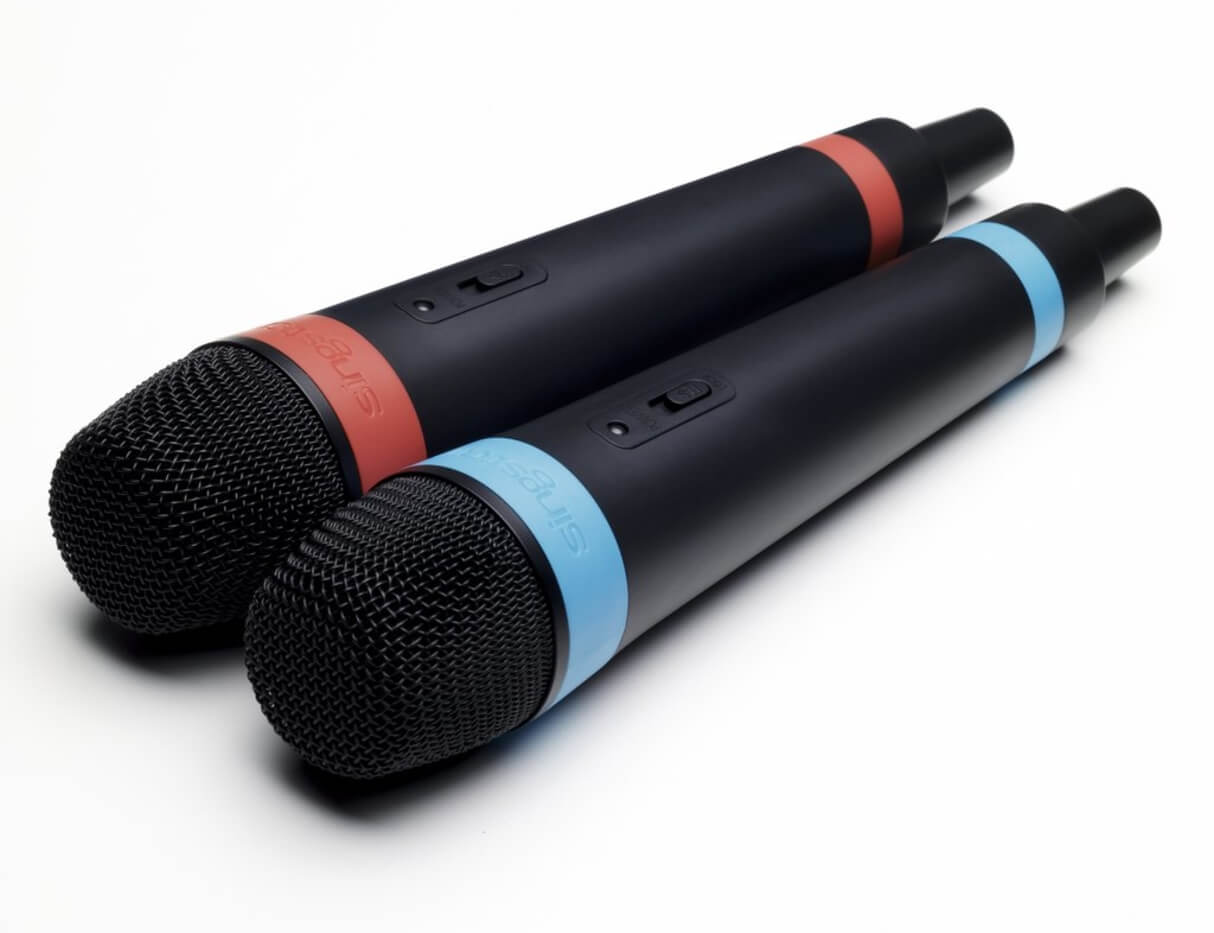
\includegraphics[width=0.4\textwidth]{Images/TechnologyReview/SingstarController.jpg}
    \centering
    \caption{Singstar microphones.}
    \label{fig:singstar}
    \vspace*{-1\baselineskip}
\end{wrapfigure}

The technology used in alternative games can, in principle, consist of almost anything. The limits in what can be done are often affiliated with the game developers’ imagination rather than the technology. A common way of creating alternative games, as described in the model in Chapter \ref{chap:what_is_alternative_game} is to explore custom-designed input or output devices. A typical example is a specific controller custom-designed for the game. Alternative games often bundle the game together with the needed controller. A concrete example of such a game is Singstar, a karaoke game where players compete to get the highest score by hitting as many notes as possible. The game includes a custom microphone, as seen in Figure \ref{fig:singstar}, that the players use when singing. By using this microphone, the player gets an increased real-world experience. Some other examples of games that use custom controllers as input are Wii Fit, Guitar Hero, and Mosquito Mania, all of which were described in Chapter \ref{chap:existing_games}. 

Augmented Reality (AR) and Virtual Reality (VR) are examples of technologies where uncommon input and output are used. The technologies have become increasingly popular in the last couple of years and are expected to continue to be available to more people in the coming years as well \citep{petrock_us_2020}. Both technologies are great platforms for developing alternative games.

VR is a technology based on simulating an environment for users where they become a part of that virtual experience. The situation could be based on a simulated version of the real world or an imaginary one. VR games give another level of immersion in the game because everything the player sees is dependent on the fictional environment. Consequently, more parts of the game experience can be controlled by the developer. An example of a player immersed in a VR game can be seen in Figure \ref{fig:playing_vr}. The corresponding in-game look for the player could be similar to the view in Figure \ref{fig:gameplay_vr}. The screenshot is captured from an actual game-play session in “The Climb” for Oculus Quest, a popular VR headset. 

\begin{figure}[H]
    \begin{minipage}[t]{.52\textwidth}
         
\includegraphics[width=0.95\textwidth]{Images/TechnologyReview/OculusQuest.jpg}
        \centering
        \caption{A person playing VR games using Oculus Quest 2.}
        \label{fig:playing_vr}
    \end{minipage}
    \hspace{0.04\textwidth}
    \begin{minipage}[t]{.43\textwidth}
        
\includegraphics[width=0.9\textwidth]{Images/TechnologyReview/TheClimbOculus.jpg}
        \centering
        \caption{Screenshot of Oculus Quest gameplay from The Climb.}
        \label{fig:gameplay_vr}
    \end{minipage}
    \vspace*{-0.5\baselineskip}
\end{figure}

AR is similar to VR, but instead of projecting elements to a simulated environment, AR uses the real world. Simulations can be created using specially developed glasses, as illustrated in Figure \ref{fig:ar_glasses}, or more commonly, with a mobile phone screen and camera. Similar to VR, AR creates another game experience than regular games. One of the most common examples of an AR game is Pokémon Go, described in Chapter \ref{chap:existing_games}.

\begin{figure}[H]
    
\includegraphics[width=0.8\textwidth]{Images/TechnologyReview/ARGlasses.jpeg}
    \centering
    \caption{AR projections in the real world using glasses.}
    \label{fig:ar_glasses}
    \vspace*{-0.5\baselineskip} 
\end{figure}

In addition to using custom controllers, AR, and VR, mobile phones are commonly used to develop alternative games. Mobile devices have a lot of sensors that developers can utilize to create a game. Also, mobile applications’ distribution is relatively simple because the popular operating systems have pre-made tools for distributing applications. The simplicity of distribution makes it more likely for users to download an application to their mobile phone than they are to buy some kind of custom device only for that game.

As mentioned in the motivation, we have focused on developing a concept that can reach as many users as possible. Mobile technology is by far the easiest and most available way to do this today. Therefore, the rest of this technology review will focus on which tools can be utilized to create the best mobile applications. The content presented in the rest of the chapter is used later to decide how we will develop our application.

\subsection{Mobile Application Development Tools}
Today, most smartphones on the market use Android or iOS as their operating system \citep{statcounter_mobile_2020}. The development can be done mainly in two different ways: native or using a cross-platform framework. The native development method uses the APIs and languages provided by Apple or Google. The cross-platform framework method uses third-party tools for creating an application that can be run on both platforms. There are strengths and weaknesses in using either of the approaches, which should be carefully considered before choosing one of them. Early decisions affect evolvability and can be hard or costly to change later \citep{ford_building_2017}. 

Alternative games often utilize the mobile phone’s sensors, such as GPS, Bluetooth, and gyroscope, as a central aspect of the game. It is, therefore, essential that the frameworks considered for alternative games have good support for accessing data from these sensors. Obtaining data from the devices is not an issue in the native approach since they are continuously updated with the latest and most detailed data available to the developer.

\subsubsection{Native Solutions}
The obvious drawback of using the native approach is that Android and iOS applications need to be developed separately. Since the native solutions for Android and iOS are based on two different programming languages, Java/Kotlin and Swift, code cannot be shared between both applications. The developers then have to implement and maintain both solutions, resulting in a “doubled” work amount.

The main strength of the native solution is that you always have access to the latest and greatest APIs provided by the companies developing the operating systems. Every time a new OS gets released, the developers have access to the latest features instantly. Availability of new features can be valuable for developers when working with special features that are not commonly utilized and creates a faster implementation loop when new features become available.

Another strength of the native solution is maturity. The APIs and tools provided are usually well documented and tested. Developing an application using this approach is not dependent on third-party developers writing documentation and updating their framework. 

If performance is critical for the application, the native approach is also preferred. While different frameworks’ performance varies significantly, based on what operations are done, native solutions are usually more performant than cross-platform frameworks \citep{biorn-hansen_empirical_2020}.

\subsubsection{Cross-Platform Solutions}
There are several variants of cross-platform solutions for mobile applications, each with different strengths and weaknesses. In this section, we will consider general-purpose and game-focused frameworks. The primary benefit of all of these approaches is the ability to share codebase between the Android and iOS applications. In theory, this should decrease development and maintenance costs since the developers can focus on only one framework. Another benefit of using cross-platform solutions is that they often utilize other languages than those supported by Google and Apple. Consequently, a developer can choose a language that fits better to their expertise.

General cross-platform frameworks focus on creating a simple application that can run on both Android and iOS. The different frameworks have their own approach, but they provide similar services. Three of the most known frameworks are \href{https://reactnative.dev}{React Native}, \href{https://flutter.dev}{Flutter}, and \href{https://dotnet.microsoft.com/apps/xamarin}{Xamarin}. When deciding on which general-purpose framework one should choose, the developer preferences are often central. But of course, it is necessary to make sure the framework supports what you plan to do in the application. General cross-platform application frameworks are suitable for most applications that do not include too much complicated graphics.

Game focused mobile framework focuses more directly on creating applications with 3D elements. The frameworks provide tools that make the creation of game elements and complex visualization easier. Thus they are perfect when working with this. However, they might be unnecessarily complex and not fit for developing applications that are simpler graphically. Two of the best-known examples of game-focused mobile frameworks are Unity and Unreal Engine.

\subsubsection{Choosing Between Native and Cross-Platform}
So whether a native approach or a cross-platform approach is best essentially comes down to the situation. If performance and access to the latest and greatest the operating system can offer, a native solution is preferable. If a shared codebase between Android and iOS or minimizing development time is crucial, a cross-platform solution is probably the way to go. And last, if you are developing 3D intensive applications, a game-specific framework should be the preferred option.

\subsection{Data Solutions}
An important aspect of game development is how the data should be stored and managed. The social element in games is crucial to create an enjoyable experience for the player \citep{sweetser_gameflow_2005}. A way of authenticating users and a central storing mechanism to keep player data is essential to provide this. There are many approaches to do this. 

Previous to cloud services, writing a custom API that handled requests from the application was the way to go. However, in the last couple of years, cloud service solutions called Backend as a Service (BaaS) are frequently used in mobile applications. The idea here is that the solution should provide all necessary backend solutions for mobile applications. All the big cloud providers, Microsoft, Google, and Amazon, offer this kind of service.

\subsubsection{Backend as a Service (BaaS)}
As mentioned above, BaaS provides all the necessary backend services for a mobile application, including authentication, storage, insights, and more. Such a solution is supposed to simplify mobile application development since the developers do not need to spend much energy on planning, creating, and maintaining a custom backend. They can instead focus on improving the application. All the big cloud providers, Microsoft, Google, and Amazon, offer similar services with \href{https://azure.microsoft.com/en-us/solutions/mobile/}{Azure Mobile Apps}, \href{https://firebase.google.com}{Firebase}, and \href{https://aws.amazon.com/amplify/}{AWS Amplify}, respectively. Choosing between these is usually subjected to taste and preferences, but the mobile application’s technology could influence the choice. For example, if Xamarin is used as a mobile application tool, Azure Mobile Apps is a great fit because Microsoft provides both. Consequently, the developer gets a lot “for free.”

In addition to the solutions from the big cloud service providers, there exist other alternatives that could be used as a replacement or extension. Two of the ones that caught our interest during this work are \href{https://parseplatform.org}{Parse} and \href{https://hasura.io}{Hasura}. Parse is an open-source backend framework. It aims to create a more straightforward backend development process and has a large community base. Parse could be a great alternative to Azure Mobile Apps, Firebase, or AWS Amplify. Hasura is a more specialized database solution. The service provides a \href{https://www.postgresql.org}{PostgreSQL} database with a \href{https://graphql.org}{GraphQL} API and built-in authentication. The main selling point for Hasura is the use of GraphQL, as opposed to the more common REST style. The main benefit of using GraphQL is the ability to specify which data properties you want to fetch, limiting the amount of data transferred, and thus is perfect for mobile applications. Hasura is not a complete BaaS and probably needs to be used in coherence with another service.

\subsubsection{Custom API}
The next approach for creating a backend solution is to write a custom API. Developing such a system is a widespread solution and was the preferred one for almost all client-server-based applications for a long time. By creating a custom API, the developer can tailor the system for the application’s needs. It is also simpler to integrate a custom API with an existing system if that is a requirement. 

There exist a large diversity of different frameworks for creating a custom API. In general, all major languages have at least one tool for developing a web API. Examples of some tools are Flask in Python, ASP.NET in C\#, and Express in Node.js.

\subsubsection{Choosing Between BaaS and Custom API}
The choice of backend solutions often depends on the developers’ preferences. If the application’s goal is to create something that does not require a lot of business logic and a complex backend, BaaS is probably the way to go. A custom API may be the best solution for larger companies where the backend needs to integrate with the existing system and contain complex logic.

\subsection{Summary}
This chapter started by briefly looking at today’s diversity in the technology used in alternative games. After that, relevant mobile application development tools were discussed and compared. This knowledge will be helpful when deciding on how the application should be developed. As explained in the motivation in Chapter \ref{chap:motivation}, we want to create a game that should “be available to as many users as possible.” Thus, a cross-platform mobile application with a BaaS data solution will probably be the preferred solution. Chapter \ref{chap:chosen_dev_technologies} presents more concrete details on which tools we chose and why they were selected.